\documentclass[12pt]{article}
\usepackage{amsmath} 
\usepackage{verbatim}
\usepackage{graphicx}    % For grafik (billederfiler)
\usepackage[T1]{fontenc} % For at blande \textsc{} med \textbf{}
\usepackage[dvipsnames,usenames]{color}
\usepackage{tabularx,colortbl,xcolor}
\definecolor{KU-red}{RGB}{144,26,30} 
\setlength{\parindent}{0mm}
\thispagestyle{empty}
\usepackage[superscript, biblabel]{cite}

\begin{document}

\begin{minipage}[b]{1.0\linewidth} 

\includegraphics[height=40mm]{KULogo}

\vspace*{-30ex}
\begin{center}
    {\Large \bf Project iBeacon} \vspace*{1ex} \\
    {\large ProjDat 2015} \vspace*{1ex} \\
    {\large Report 1} \vspace*{1ex} \\
    {\large March 23, 2015} \vspace*{1ex} \\
    \ \\
    
    {\large Emil Slot Arakelian Jensen - 170494} \vspace*{1ex}\\
	{\large Samuel Korn - 101186} \vspace*{1ex}\\
	{\large Mark Jay Nielsen - 250694} \vspace*{1ex}\\
	{\large Rune Bjerg Ono - 180187} \vspace*{1ex}\\
	\ \\
	
	{\large TA: Kasper Passov} \vspace*{1ex} \\
\end{center}

\vspace*{-3pt}
{\color{KU-red}\hrule}
\end{minipage}


\newpage

\tableofcontents










\newpage
\section{Problem definition}

\subsection{Overview}

The following text, is the original description of one of the many projects made available to us from the company Shape A/S.\\

\textit{\textbf{How many people are in the office?}\\
Use iBeacons to determine the amount of people currently in the office. \\
. . .
Using iBeacons we would like to make an app that registers whenever the user enters or leaves our office. . . . This could e.g. be used to adjust the heating, automatically lock the doors and turn off the lights when the last person leaves, predict when we need to order more or less lunch, or simply to check whether a certain person is currently at the office.} \cite{shape_ws}\\

These particular iBeacon devices are made by a company called Estimote, and are described as \textit{. . . small wireless sensors that you can attach to any location or object. They broadcast tiny radio signals which your smartphone can receive and interpret, unlocking micro-location and contextual awareness.} \cite{estimote_ws}\\

On March the 12th, we had a meeting with S\o ren Ulrikkeholm, who is the developer responsible for student contact at Shape. We talked about the different projects and realistic acceptance criteria, taking into account our limited experience. We settled on the aforementioned project, because it was deemed the most appropriate for our level of skill, as well as being the one in which Shape had the most interest.\\

S\o ren explained that the company's biggest interest is learning how to use iBeacons with Android, while aggregation of the data and application of machine learning and data visualization are secondary objectives. We have decided to split the project into two development phases.\\



\subsection{Problem statement}

\subsubsection{Problem domain}
Our primary focus is on the first development phase, which consists of developing an app for Android that registers individual users entering and leaving the office space.\\

The second development phase consists of developing the backend for the system and integrating it with the app, in order to aggregate the data from users entering and leaving the office in a database.\\



\subsubsection{Solution domain}
Our client will be using this system in their office, with the intention of aggregating data on employees entering and leaving the office. The plan is for them to apply machine learning and data visualizations to this data to discover usage patterns allowing them to implement automatic control of various functions within the office.



\subsubsection{Functional requirements}
The app must be able to register an iBeacon in the near vicinity.\\
The app must register a user entering or leaving the office.\\
The app must communicate with a database to collect this data.\\



\subsubsection{Non-functional requirements}
The app must be written in Java and XML for the Android operating system.\\
The app must be simple to use.\\



\subsubsection{Deadlines}
So far we only have a couple of deadlines.\\
\textbf{March 22:} Delivery of problem definition to client.\\
\textbf{June 8:} Delivery date for finished product.\\










\section{Initial Software Project Management Plan}

\subsection{Work breakdown}
As of now, we are only in the initial phase of designing our app, therefore the current management plans and schedules are rough drafts.\\
We have made a very rough draft of a partial work breakdown structure (see figure 1) for the project, but it is still very general and not very detailed.\\

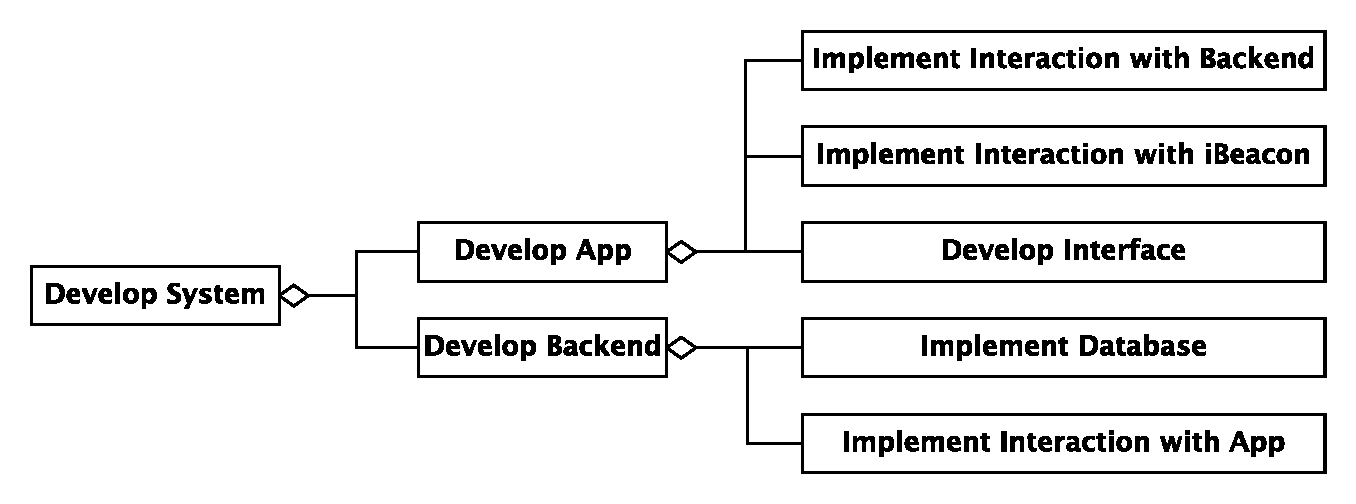
\includegraphics[scale=0.6]{work_breakdown}\\
\textbf{Fig. 1:} Partial work breakdown structure for the project.\\



\subsection{Roles and responsibilities}

\subsubsection{Internal roles}
With regards to the development of the system we have not appointed any specific roles or responsibilities. We are a group of only four people and are confident that we do not need to appoint a project manager to supervise the remaining three. We will however, later on in the development, create detailed schedules and individual deadlines for smaller assignments, which we will use to keep track of our progress rather than having a single person be manager. This approach is not quite the same as mentioned in our textbook \cite{OOSE}, however, given the size of our team we believe we can manage this project together.\\
See figure 2 for a skill matrix for our group.\\

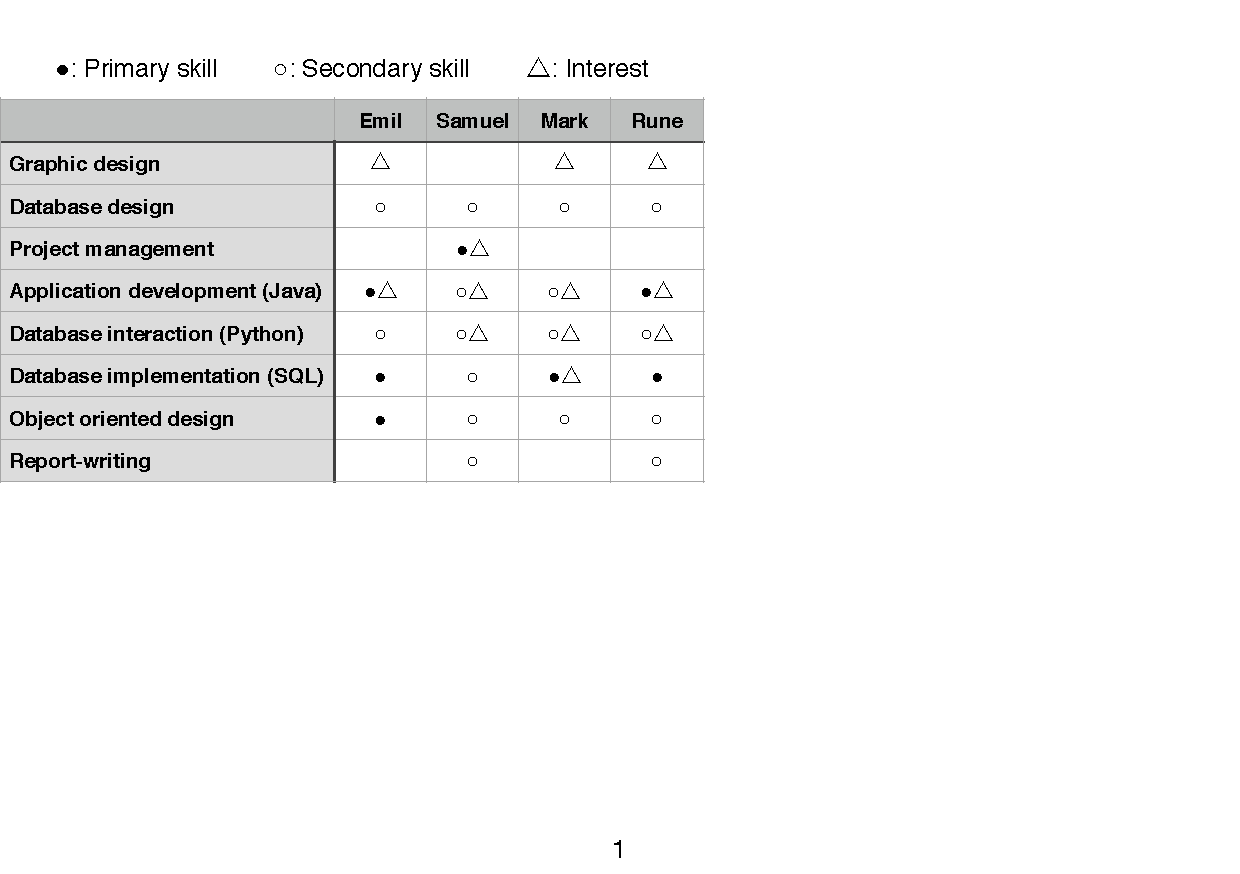
\includegraphics[trim=0 64mm 0 0, clip]{skill_matrix}\\
\textbf{Fig. 2:} Skill matrix.\\


\subsubsection{External roles}
With regards to external roles, Rune is responsible for communication with the client and Samuel is responsible for communication with our appointed TA, Kasper Passov.\\



\subsection{Project schedule}
\textbf{March 16 - March 22:} Problem definition.\\
\textbf{March 23 - April 5:} Initial design phase.\\
\textbf{April 5 - June 7:} Main development phase.\\



\subsection{Budget}
We do not plan to have any expenses tied to the development of our project, nor does the development software pose any costs. Shape A/S will provide us with access to the iBeacon devices.\\


\subsection{Risks}
INSERT\\










\section{Initial software architecture}

We are developing the system from scratch rather than building on top of existing software. As we are developing the app for Android, it will be programmed mainly in Java as well as XML. We expect to be implementing the backend of the system as some sort of SQL database.\\










\newpage
\section{Project Agreement definition}

The following is a translation of the Project Agreement definition, agreed upon by both our client and ourselves:\\

Together with Shape A/S we have chosen to work on project 5 from their website www.shape.dk/projects. The project consists of developing an app for the Android and iOS operating systems that, using an iBeacon device, collects data showing how many people are present in their office at a given time. This data is collected with the intention of finding usage patterns which could potentially be used for automatic control of a number of functions in the office (turning the lights on/off, regulating the room temperature etc.).\\

During our meeting with the client on March 12th we discussed how the project can be split into 3 development phases. First phase involves designing and developing an app which collects data fra an iBeacon. Second phase is to integrate the app with a backend database that stores all the collected data, and the third phase revolves around the use of the stored data for data visualizations and machine learning purposes.\\

An app for both iOS and Android would be too much for us to handle, which is why we have agreed to only develop the app for Android. Our limited programming experience means that we will be focusing solely on the first two development phases, i.e. we will only be designing and developing the app and implementing the database. A temporary schedule follows.\\

\textbf{March 16 - March 22:} Problem definition.\\
\textbf{March 23 - April 5:} Initial design phase.\\
\textbf{April 5 - June 7:} Main development phase.\\
\textbf{June 8:} Product delivery date.\\

We have made an arrangement with Shape A/S to be able to work on the project in their office one day of every week.\\

Our next meeting with the client will be on March 25th at 10 o'clock, where we will have our first look at the iBeacon device.\\

Aside from their time Shape A/S will have no expenses tied to this project.










\section{Project establishment}

Neither of us have been working with iBeacons nor Android apps before. We expect to learn more about application development and specifically how to implement iBeacons in such applications. We might run into some problems when developing our application and/or have some problems implementing interaction with iBeacons.\\

Our client's interest in this project is to receive a finished product for use in their office. The interest of our group is also to gain experience working in a corporate setting as well as extending our software development skills. No other parties have an interest in this project.\\

In addition to meeting once a week at the office, we plan to dedicate at least one more day a week to work on the project. At this current point in time we do not know how much time needs to be used on the project, and the plan is therefore only temporary.










\newpage
\section{Exercises}

\subsection{1-6.}
\textbf{Specify which of these statements are functional requirements and which are
nonfunctional requirements}

Functional requirements:\\
- "The TicketDistributor must enable a traveler to buy weekly passes."\\
- "The TicketDistributor must always be available."\\
- "The TicketDistributor must provide a phone number to call when it fails."\\

Nonfunctional requirements:\\
- "The TicketDistributor must be written in Java."\\
- "The TicketDistributor must be easy to use."\\



\subsection{1-8.}
\textbf{In the following description, explain when the term account is used as an application domain concept and when as a solution domain concept:}\\
"...managing bank accounts for mobile costumers." - It is used as an application domain concept, saying what it is supposed to do. 
"...provide access to the accounts when the..." - It is used the same way as before. 
"One proposal is that accounts are made available on the mobile computer..." - Here it is used as a solution domain concept, as it is a possible solution to be evaluated. 
"...the accounts show the amounts from the last connected session." - It is used in connection with the previous use.\\



\subsection{2-6, 2-7, 2-9.}
\textbf{Draw a class diagram representing a book. Add multiplicity to the class diagram you produced in Exercise 2-6. Extend the class diagram to include attributes.}\\

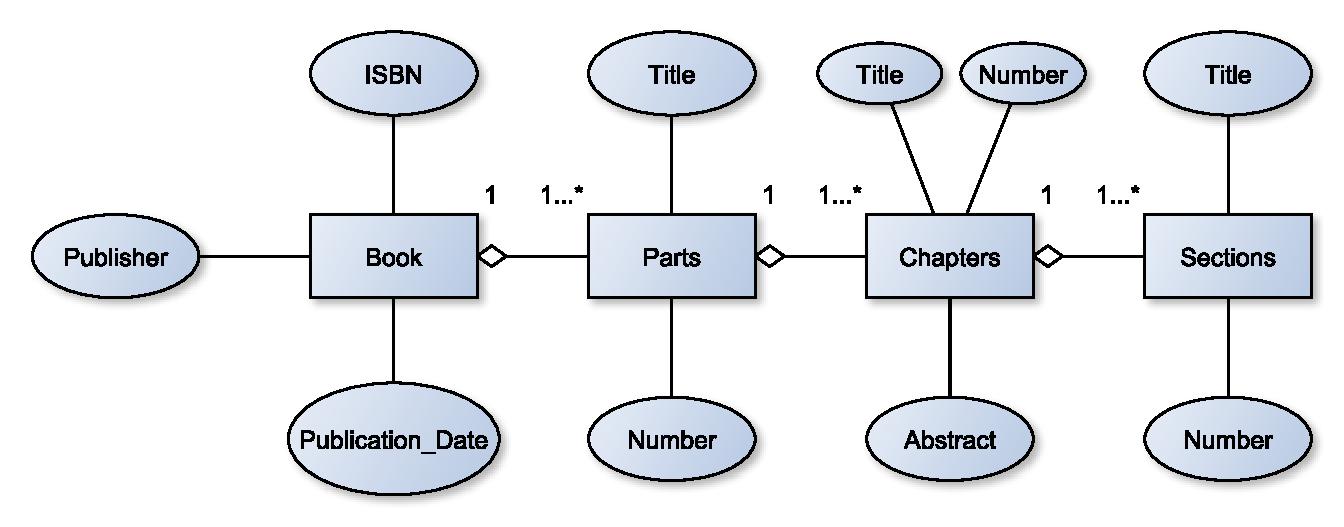
\includegraphics[height=50mm]{2-6}\\
\textbf{Fig. 3:} Class diagram for exercise 2-6, 2-7 and 2-9.



\subsection{2-10.}
\textbf{Add an abstract class and an inheritance relationship to factor out these two attributes into the abstract class}\\

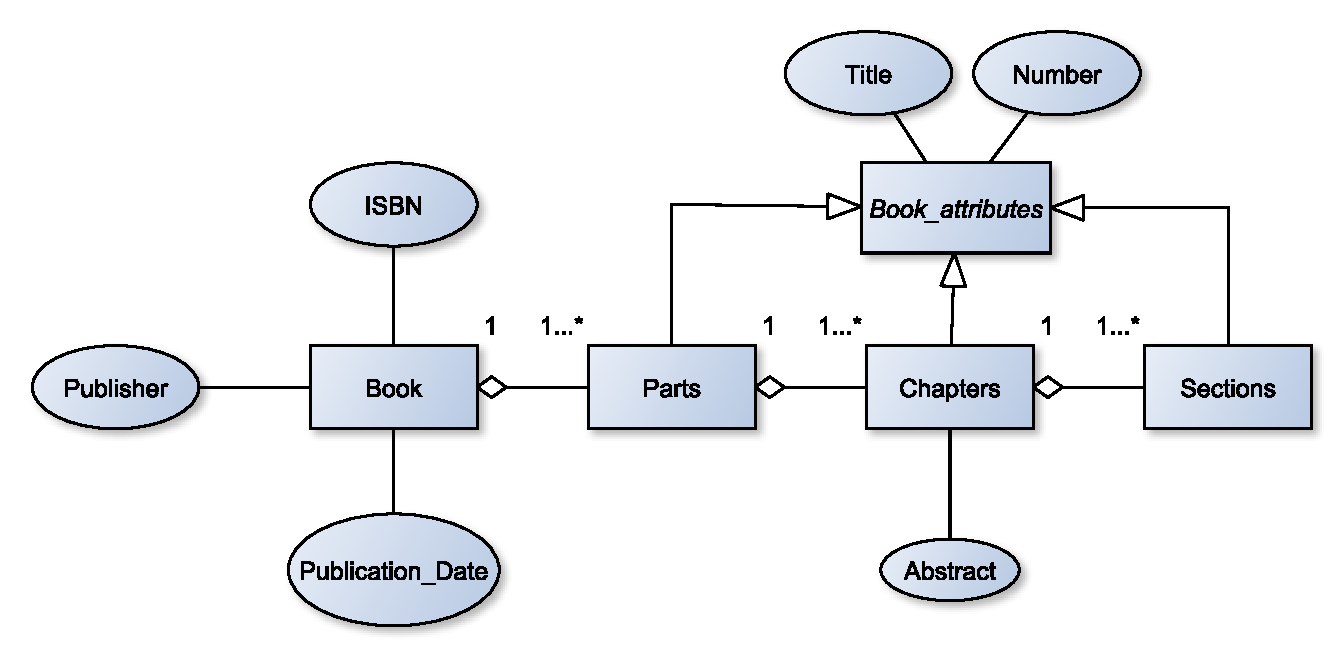
\includegraphics[height=70mm]{2-10}\\
\textbf{Fig. 4:} Altered class diagram for exercise 2-10.



\newpage
\subsection{5-3.}
\textbf{Arrange the objects listed in Exercises 5-1 and 5-2 horizontally on a sequence diagram.}\\
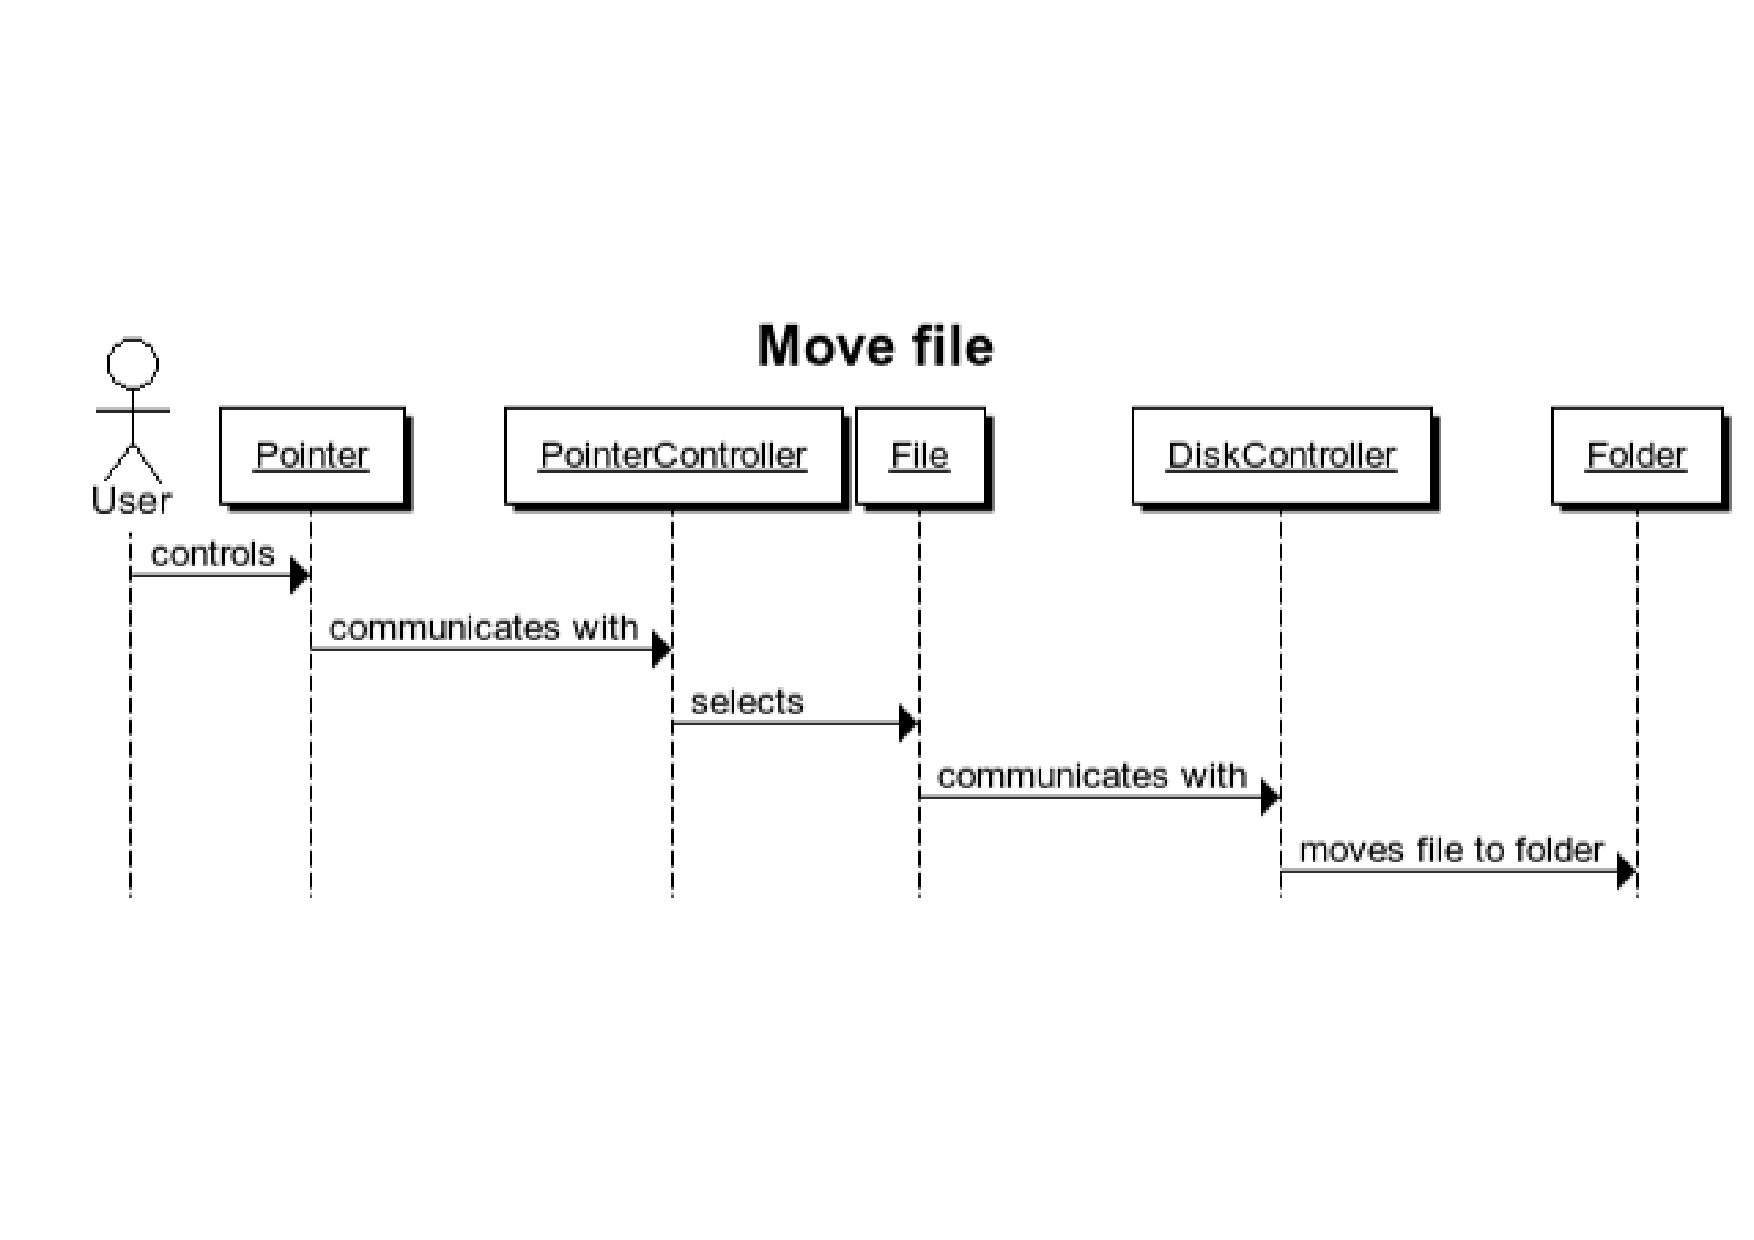
\includegraphics[scale=0.5]{5-3}\\
\textbf{Fig. 5:} Sequence diagram for exercise 5-3.



\newpage
\subsection{7-1}
\textbf{Draw a UML deployment diagram representing the hardware/software mapping.}\\

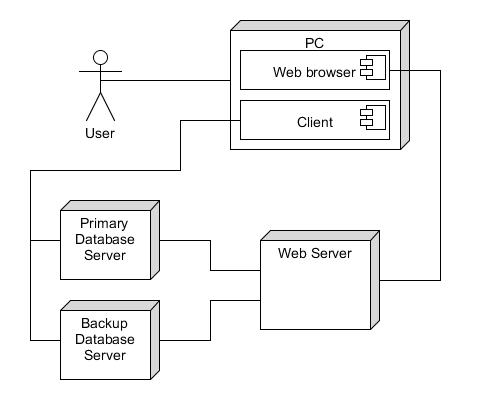
\includegraphics[scale=0.7]{7-1}\\
\textbf{Fig. 6:} Deployment diagram for exercise 7-1.










\newpage
\begin{thebibliography}{9}

\bibitem{shape_ws}
http://www.shape.dk/projects

\bibitem{estimote_ws}
http://www.estimote.com
  
\bibitem{OOSE}
Bruegge \& Dutoit (2010), Object-Oriented Software Engineering - using UML, Patterns and Java, Third edition, Pearson 2010. Page 611.

\end{thebibliography}

\end{document}
